%
% 21-geschlossen.tex -- Wegintegrale über geschlossene Wege
%
% (c) 2026 Prof Dr Andreas Müller
%
\subsection{Wegintegrale über geschlossene Wege}
%
% fig-residuum.tex
%
% (c) 2026 Prof Dr Andreas Müller
%
\begin{figure}
\centering
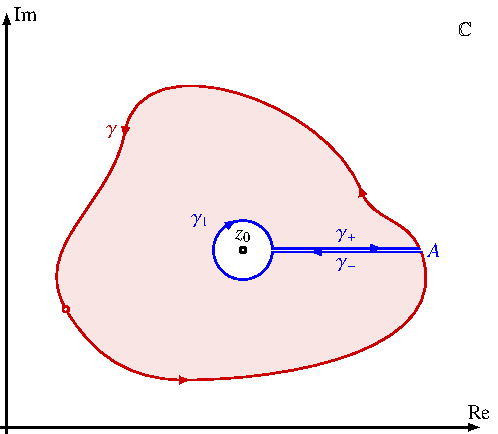
\includegraphics{chapters/030-integration/images/residuum.pdf}
\caption{Herleitung des Integralsatzes.
Der Weg $\gamma$ wird durch die Segmente $\gamma_-$, $\gamma_1$ und
$\gamma_+$ zu einem Weg ergänzt, der das hellrote Gebiet berandet,
in dem die Funktion $f(z)/(z-z_0)$ holomorph ist.
\label{buch:integration:homologie:fig:residuum}}
\end{figure}
%
Nach dem Satz~\ref{buch:integration:wegintegral:satz:zusammenziehbar}
von Abschnitt~\ref{buch:integration:wegintegral:subsection:homotopie}
verschwindet das Integral einer holomorphen Funktion entlang eines
zusammenziehbaren Weges.
Wir betrachten jetzt eine holomorphe Funktion $f$ in einem Gebiet $U$
und einen Punkt $z_0\in U$
und einen Weg $\gamma$, der den Punkt $z_0\in U$
einmal im Gegenuhrzeigersinn umläuft
(siehe Abbildung\ref{buch:integration:homologie:fig:residuum}).
Die Funktion
\[
f_0
\colon
U\setminus\{z_0\}
\to
\mathbb{C}
:
z
\mapsto
\frac{f(z)}{z-z_0}
\]
ist immer noch holomorph.
Der Weg $\gamma$ ist jetzt im Definitionsgebiet $U\setminus \{z_0\}$
der Funktion $f_0$ nicht mehr zusammenziehbar, er müsste über den Punkt
$z_0$ hinweggezogen werden, wo die Funktion $f_0$ nicht definiert ist.
Man kann also nicht erwarten, dass das Integral von $f_0(z)$ über
den Weg $\gamma$ verschwindet.
Vielmehr gilt der folgende, viel überraschendere Satz.

\begin{satz}[Cauchy]
\label{buch:integration:satz:residuensatz}
\index{Satz!Cauchy-Integralformel}%
\index{Cauchy-Integralformel}%
Sei $f\colon U\to\mathbb{C}$ holomorphe Funktion und $\gamma\colon I\to U$
ein geschlossener Weg, der den Punkt $z_0$ einmal im Gegenuhrzeigersinn
umläuft.
Dann gilt
\begin{equation}
f(z_0)
=
\frac{1}{2\pi i}
\oint_{\gamma} \frac{f(z)}{z-z_0}\,dz.
\label{buch:integration:eqn:residuensatz}
\end{equation}
\end{satz}

\begin{proof}
Die Berechnung des Integrals
\eqref{buch:integration:eqn:residuensatz}
wird dadurch erschwert, dass der Weg $\gamma$ den Punkt $z_0$
umläuft, der nicht im Definitionsgebiet liegt.
Wir ergänzen ihn daher zu einem geschlossenen Weg, der ein
ganz in $U\setminus\{z_0\}$ liegendes Gebiet berandet.
Dazu fügen wir beim Punkt $A$ die in 
Abbildung~\ref{buch:integration:homologie:fig:residuum}
blau eingezeichneten Wegstücke $\gamma_-$, $\gamma_1$ und $\gamma_+$ 
ein.
In der Zeichnung haben die Wege $\gamma_-$ und $\gamma_+$ aus Gründen
der Darstellung einen kleinen Abstand, in Wahrheit sollen diese beiden
Wegstücke bis auf die Durchlaufrichtung identisch sein.
Nach dem Homotpiesatz gilt jetzt
\begin{equation}
\int_{\gamma
\cdot
\gamma_-
\cdot
\gamma_1
\cdot
\gamma_+
}
\frac{f(z)}{z-z_0}\,dz
=
0,
\label{buch:integration:residuensatz:eqn:proof1}
\end{equation}
weil die Funktion im hellrot gefärbten Gebiet, welches vom zusammengesetzten
Weg berandet wird, holomorph ist.

Die Wegstücke $\gamma_-$ und $\gamma_+$ werden in entgegengesetzter 
Richtung durchlaufen.
Verkettet bilden sie einen zusammenziehbaren Weg im Definitionsgebiet
der der Funktion $f_0$.
Die Wegintegrale über diese beiden Teilstücke heben sich also weg.

Vom Integral auf der linken Seite von
\eqref{buch:integration:residuensatz:eqn:proof1}
bleiben jetzt nur noch die Integrale über die beiden Wegstücke
$\gamma$ und $\gamma_1$,
die sich wegen \eqref{buch:integration:residuensatz:eqn:proof1}
ebenfalls wegheben müssen.
Es gilt also
\begin{equation}
0
=
\int_{\gamma+\gamma_1}
\frac{f(z)}{z-z_0}
\,dz
=
\oint_{\gamma}
\frac{f(z)}{z-z_0}
\,dz
+
\oint_{\gamma_1}
\frac{f(z)}{z-z_0}
\,dz
\quad\Rightarrow\quad
\oint_\gamma
\frac{f(z)}{z-z_0}
\,dz
=
-
\oint_{\gamma_1}
\frac{f(z)}{z-z_0}
\,dz.
\label{buch:integration:residuensatz:eqn:proof2}
\end{equation}

Zur Berechnung des Integrals über $\gamma_1$ verwenden wir die
Parametrisierung
\[
\gamma_1
\colon
I
\to
\mathbb{C}
:
t
\mapsto
\gamma_1(t)
=
z_0
+
re^{-2\pi i t}.
\]
mit der Ableitung 
\[
\dot{\gamma}_1(t)
=
-2\pi i r e^{-2\pi it}.
\]
Damit können wir das Wegintegral über $\gamma_1$ berechnen und
erhalten
\begin{align}
\int_{\gamma_1}
\frac{f(z)}{z-z_0}\,dz
&=
\int_0^1
f_0(\gamma_1(t))\cdot \dot{\gamma}_1(t)\,dt
\\
&=
\int_0^1
\frac{f(z_0+re^{-2\pi it})}{e^{-2\pi it}}
\cdot(-2\pi i r e^{-2\pi it})
\,dt
\notag
\\
&=
-2\pi i
\int_0^1
f(z_0+re^{-2\pi it})
\,dt.
\notag
\intertext{Nach dem Homotpiesatz~\ref{buch:integration:satz:homotopie} 
bleibt das letzte Integral gleich, wenn der Radius $r$ des kleinen
Kreises $\gamma_1$ verkleinert wird.
Insbesondere gilt im Grenzübergang $r\to 0$}
\int_{\gamma_1}
\frac{f(z)}{z-z_0}\,dz
&=
\lim_{r\to 0}
\biggl(
-2\pi i
\int_0^1
f(z_0+re^{-2\pi it})
\,dt
\biggr)
\notag
\\
&=
-2\pi i
\int_0^1
f(z_0)\,dt
=
-2\pi if(z_0).
\label{buch:integration:residuensatz:eqn:proof3}
\end{align}
Indem man das Resultat
\eqref{buch:integration:residuensatz:eqn:proof3}
in
\eqref{buch:integration:residuensatz:eqn:proof2}
einsetzt, findet man jetzt
\[
\oint_\gamma
\frac{f(z)}{z-z_0}
\,dz
=
2\pi if(z_0)
\qquad\Rightarrow\qquad
f(z_0)
=
\frac{1}{2\pi i}
\oint_\gamma
\frac{f(z)}{z-z_0}
\,dz.
\]
Damit ist der Satz bewiesen.
\end{proof}

Der Satz sagt, dass die Werte der holomoprhen Funktion $f(z)$ im
Inneren des Weges vollständig durch die Werte der Funktion auf
dem Weg $\gamma$ bestimmt sind.
